\chapter{大规模LEO卫星网络分布式管控架构及关键技术}
\label{chap:arch-techniques}

\section{引言}

大规模 LEO 卫星网络凭借低传输时延、广域覆盖和灵活组网能力，已成为未来空天地一体化信息网络的重要组成部分。然而，星座规模持续扩张、星间拓扑高速变化、星上资源受限以及控制链路不稳定等因素，使传统集中式或依赖全网状态同步的管控方式难以适配大规模星座的实时网络控制需求。为此，本章围绕大规模 LEO 卫星网络的分布式管控问题，首先对集中式、传统分布式和基于 AI 的纯分布式管控架构进行对比分析，随后从端到端传输流程出发梳理网络状态感知、用户接入与切换、无线资源调度和可靠传输等关键技术的功能定位。在此基础上，本章进一步总结时空图学习和多智能体强化学习在分布式状态感知与资源调度中的基础作用，为后续章节的具体技术设计奠定架构与方法基础。

\section{大规模LEO卫星星座管控架构}
\subsection{典型管控架构对比}
\label{sec:ch2_arch_comparison}

大规模 LEO 卫星星座的网络管控机制须在动态拓扑、受限星间链路资源与有限星上计算能力之间权衡。围绕控制闭环位置、状态视图范围与状态同步开销，现有卫星网络管控架构可归纳为三类：集中式管控架构、传统分布式管控架构以及基于人工智能（AI）的纯分布式管控架构。集中式架构由地面控制中心、高轨卫星或逻辑集中控制器维护全局或域内状态视图；传统分布式架构不设置中心控制实体，但仍依赖全网链路状态同步维护一致拓扑视图；纯分布式架构进一步将决策闭环压缩至星上节点本地或有限跳邻域，使每颗卫星仅依据本地观测和邻域遥测完成网络控制决策。

为对比三类管控架构的运行机制，本章以星间路由为例展开分析。星间路由的目标是在给定星座拓扑、星间链路状态、节点负载状态以及端到端业务需求的条件下，为业务数据流确定多跳星间链路转发路径。由于 LEO 卫星网络的节点位置、星间可见关系与链路质量随轨道运动持续变化，路由机制不仅须刻画时变网络拓扑，还须在有限控制信令与星上计算资源约束下完成网络状态获取、路径计算与转发表更新。已有研究表明，星间链路结构、控制平面架构和星上处理能力是影响大规模 LEO 星座路由设计的重要因素~\cite{Radhakrishnan-PhysicalNetwork-ComSurveys2016,chen-AnalysisISLLEO-TVT21,ji-SatOpt-TWC22,zhang-distributedSat-SCIS2025}。对应于上述三类管控架构，星间路由可形成集中式路由、传统分布式路由以及基于 AI 的纯分布式路由三种典型形态；其差异不在于单个路由算法优劣，而在于状态信息在哪里汇聚、控制闭环在哪里完成，以及同步开销如何随星座规模增长，其基本控制流向如图~\ref{fig:routing_architectures} 所示。

\begin{figure}[!htp]
    \centering
    \begin{subfigure}[t]{0.32\textwidth}
        \centering
        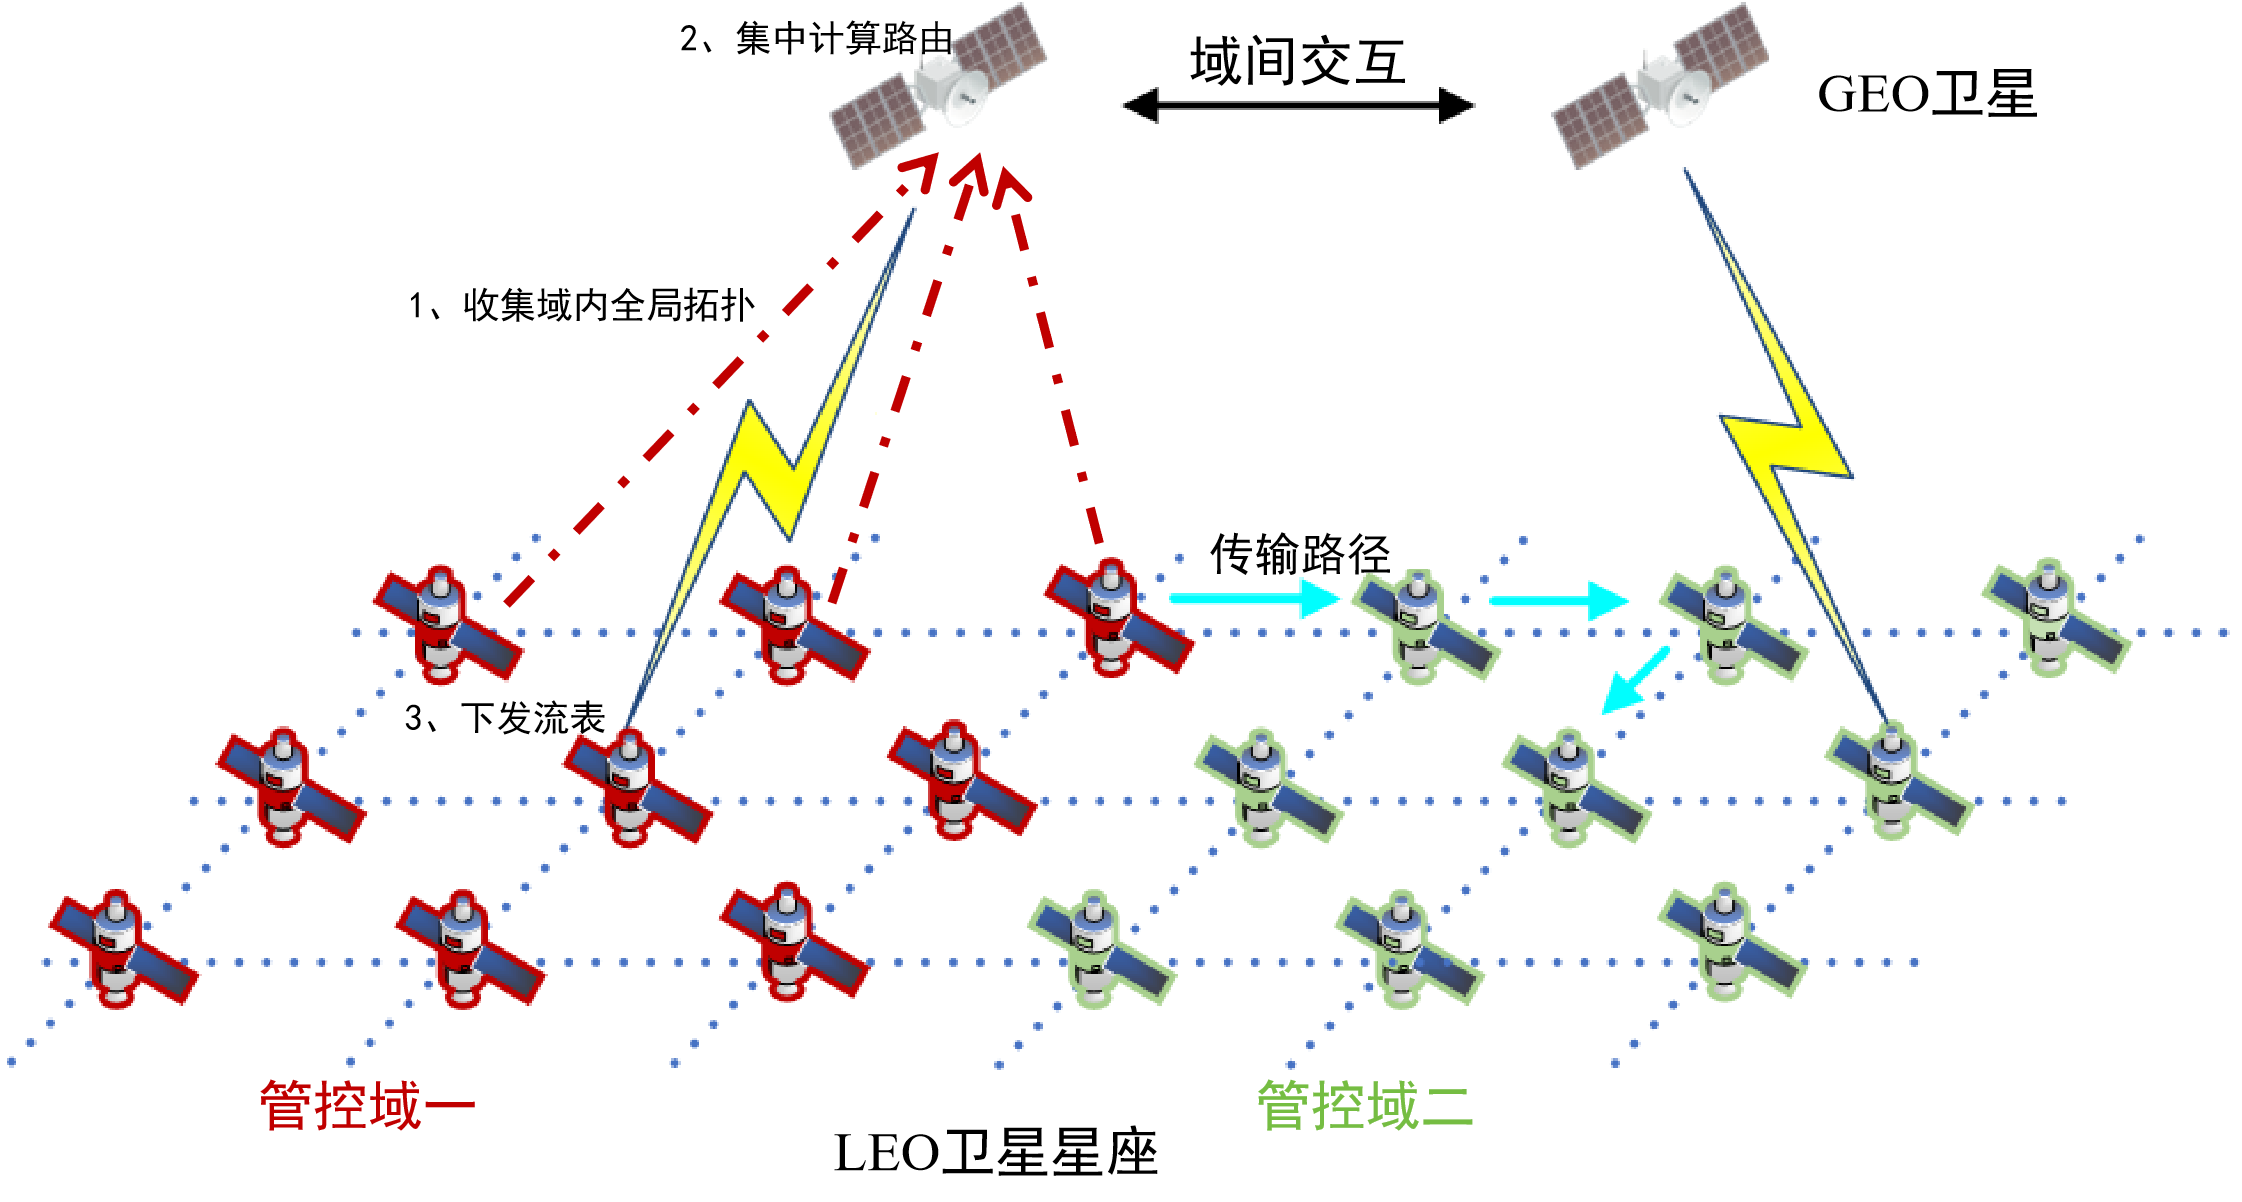
\includegraphics[width=\linewidth]{figures/chapter2/3_routing_SDN}
        \caption{集中式路由管控}
        \label{fig:routing_sdn}
    \end{subfigure}
    \hfill
    \begin{subfigure}[t]{0.32\textwidth}
        \centering
        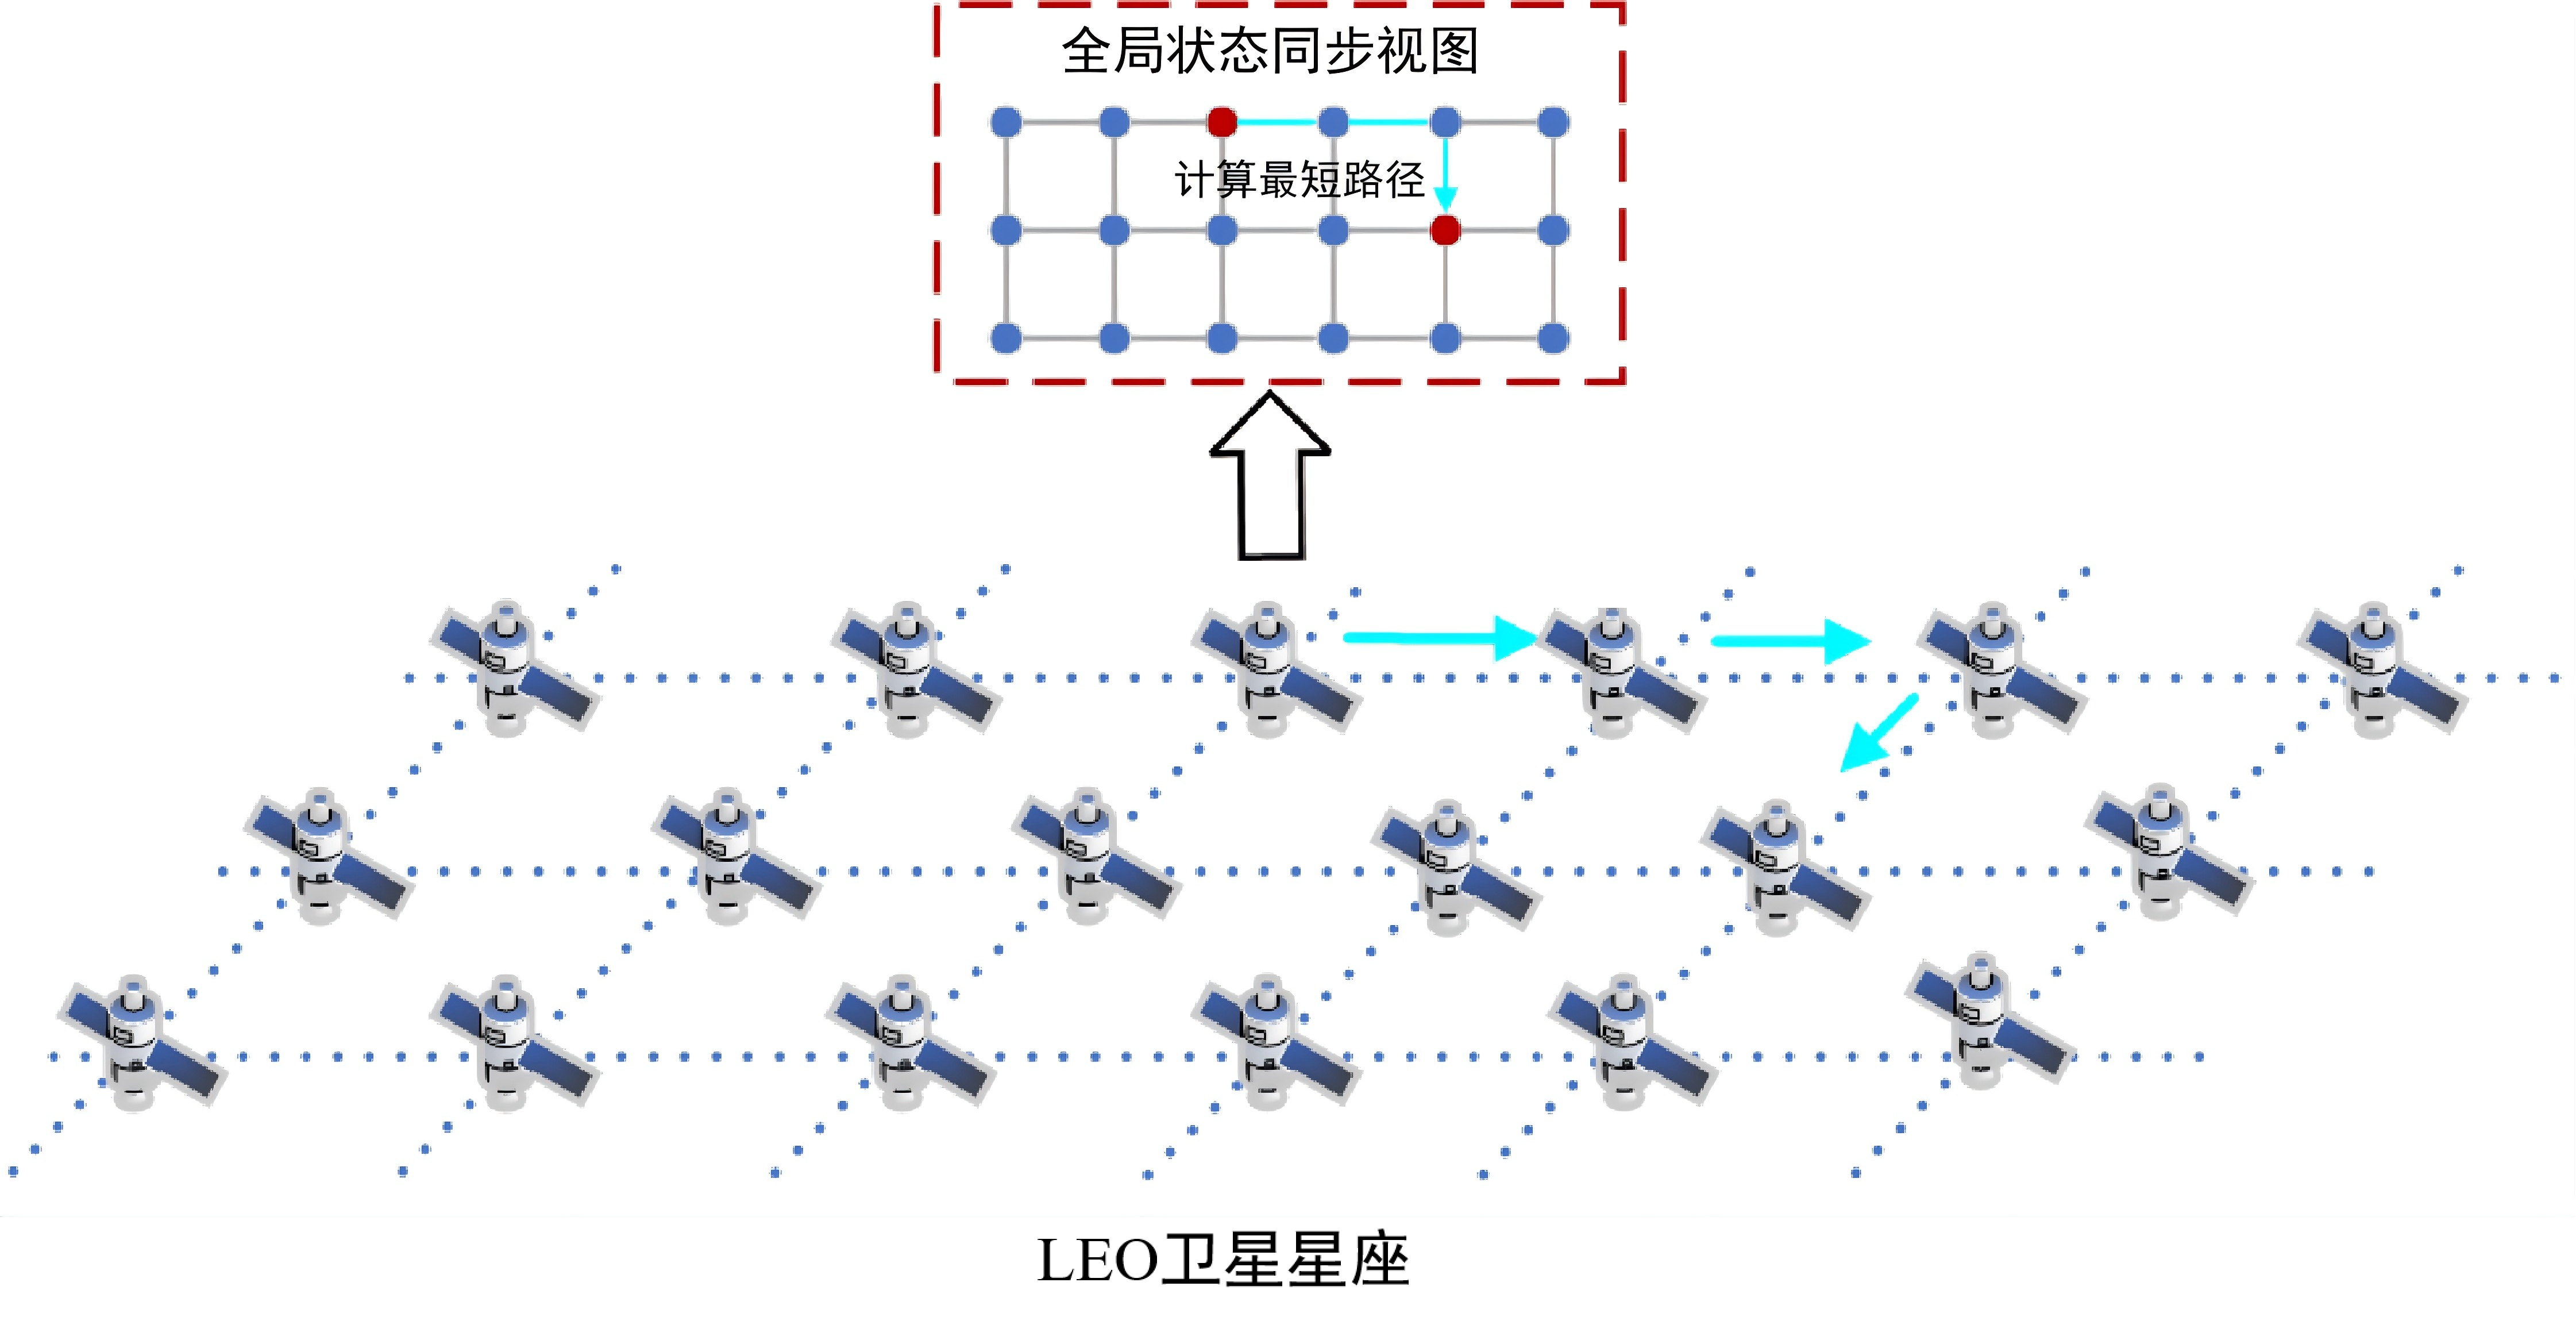
\includegraphics[width=\linewidth]{figures/chapter2/2_routing_ospf}
        \caption{传统分布式路由管控}
        \label{fig:routing_trad}
    \end{subfigure}
    \hfill
    \begin{subfigure}[t]{0.32\textwidth}
        \centering
        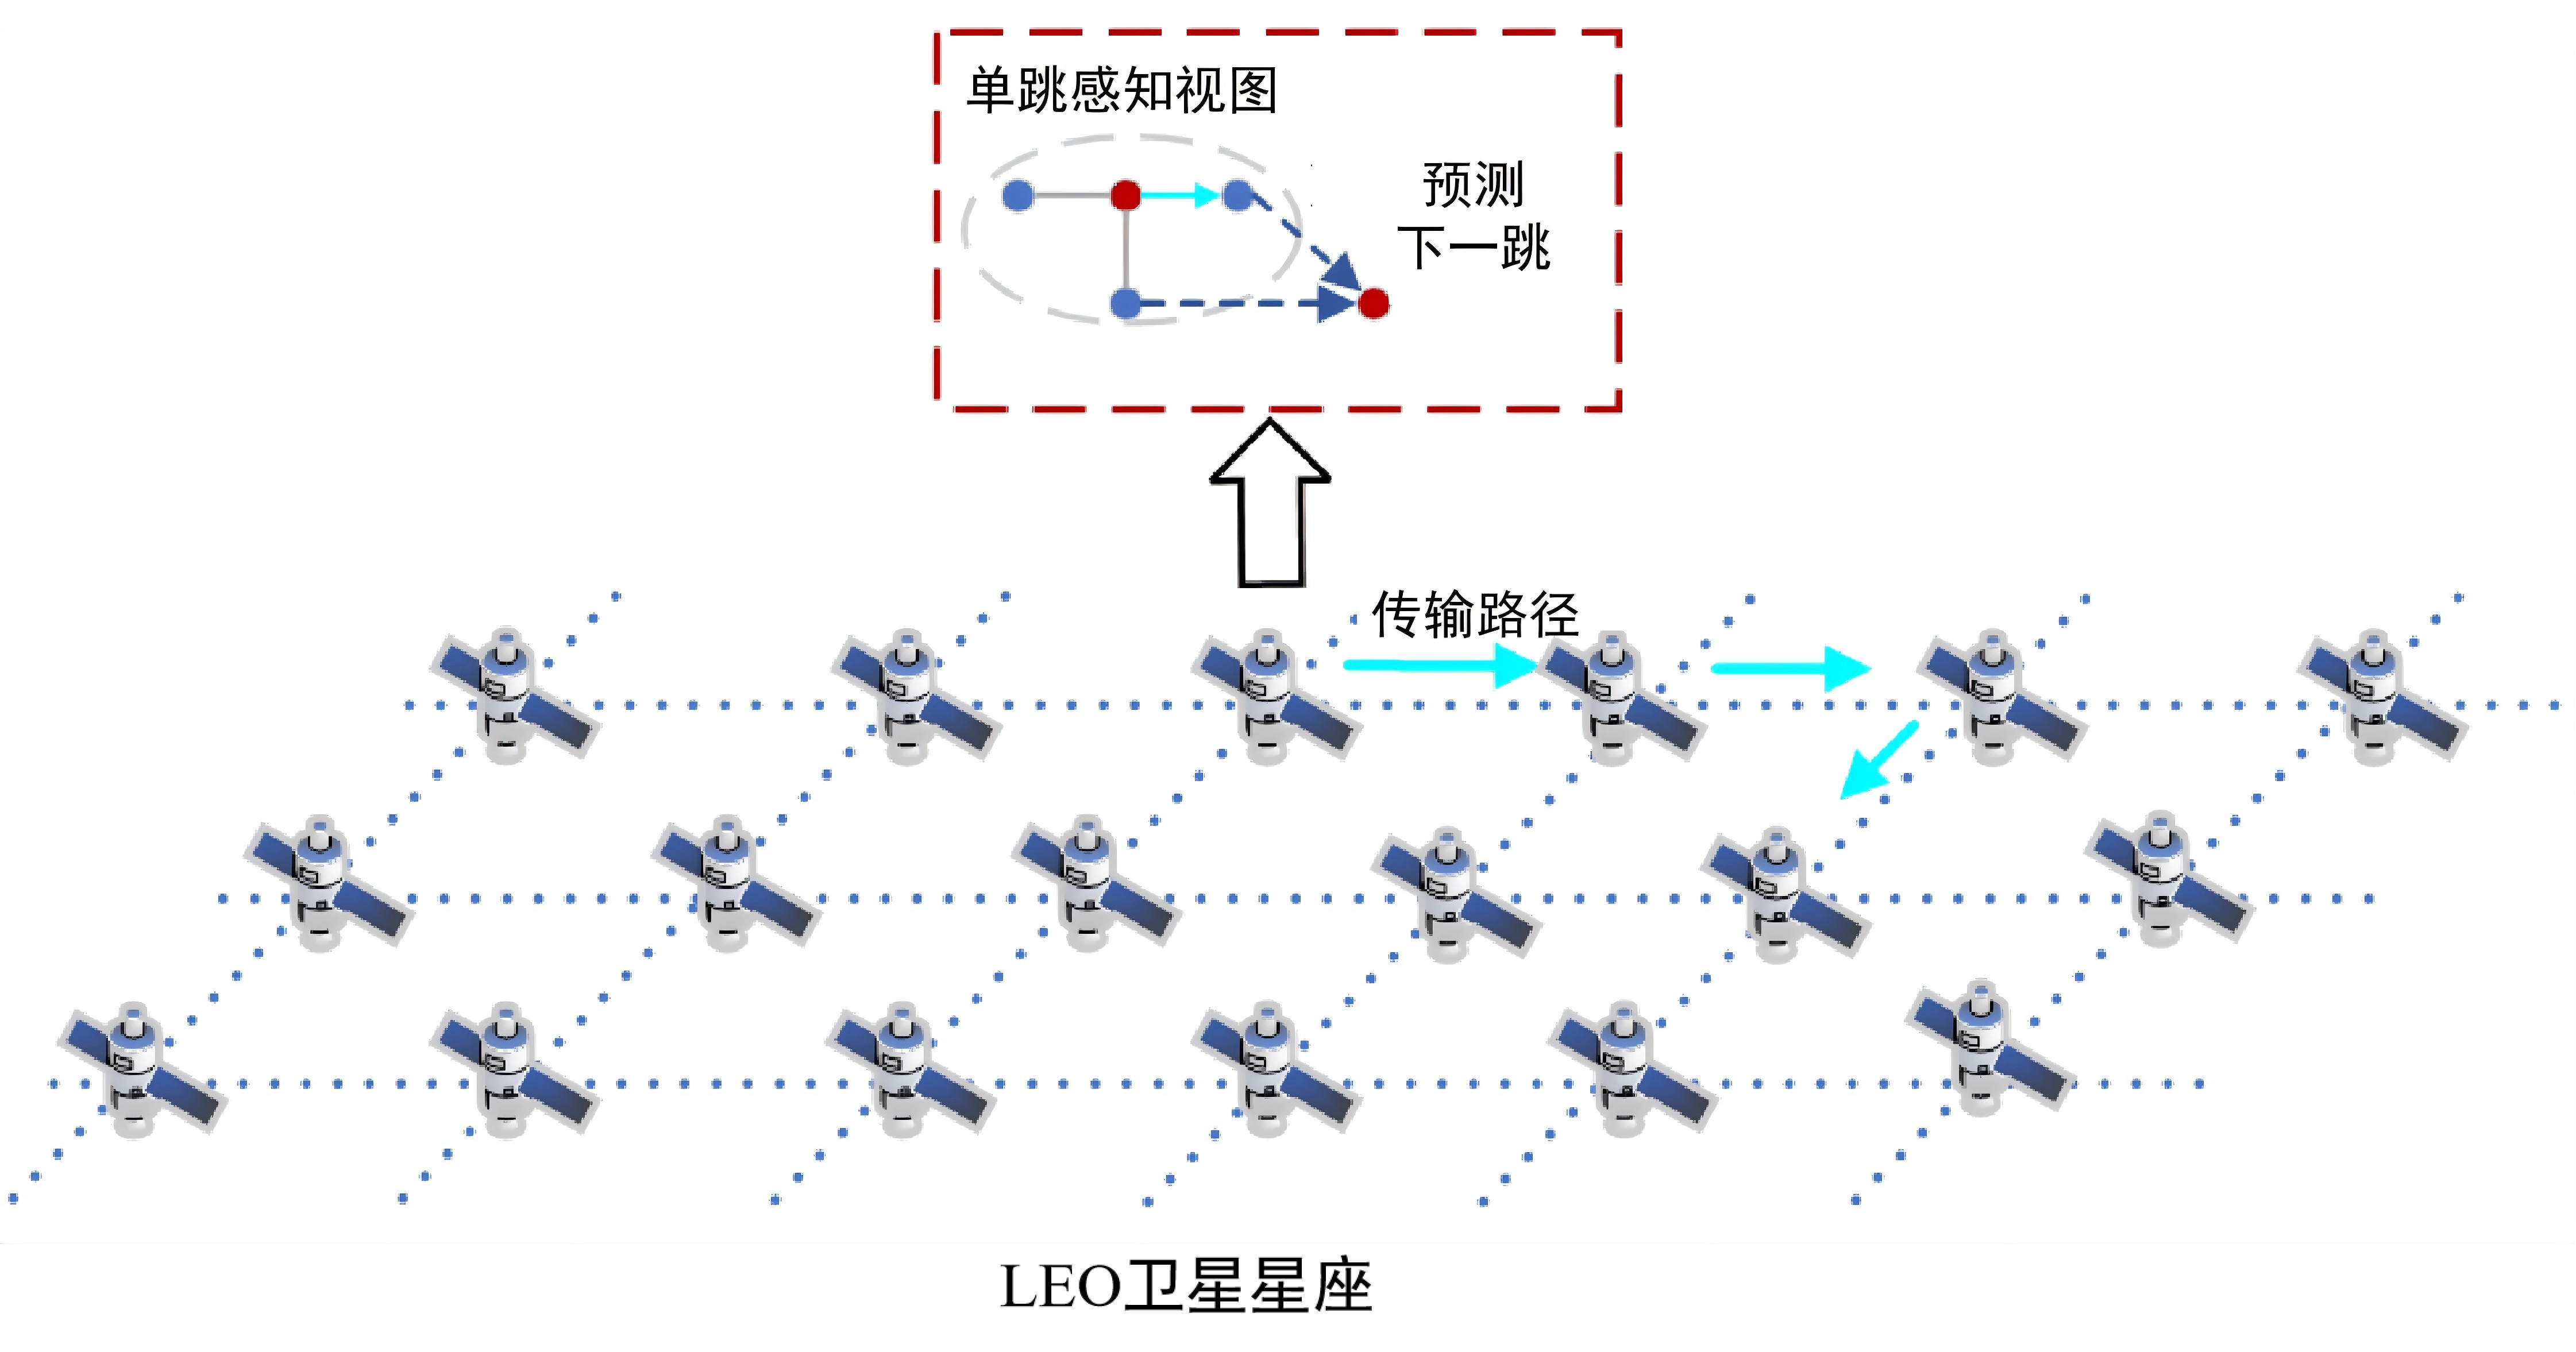
\includegraphics[width=\linewidth]{figures/chapter2/1_routing_drl}
        \caption{基于 AI 的纯分布式路由管控}
        \label{fig:routing_drl}
    \end{subfigure}
    \caption{面向 LEO 卫星星座的典型星间路由管控架构}
    \label{fig:routing_architectures}
\end{figure}

集中式路由架构对应集中式网络管控模式，如图~\ref{fig:routing_sdn} 所示。在该架构下，路由决策功能通常部署于地面控制中心、高轨卫星、空间域控制节点或逻辑集中控制器中。LEO 卫星主要作为数据面转发节点，负责本地状态采集、分组转发和转发表项执行，并将拓扑连接关系、星间链路质量、队列负载和业务需求等信息上报至控制实体。控制实体依据汇聚得到的全局或域内状态视图进行路径计算、流量工程和转发策略生成，再将路由表、流表或控制策略下发至相关卫星节点。该类架构通常与 SDN 结合，通过控制面与数据面分离提升路由策略可编程性~\cite{kumar-fybrrlink-tnsm2022,zheng-SDNinSpace-TON24,choi-SDNVirt-IoTJ2025}。集中式路由的优势在于状态视图较完整，局限在于状态上报、集中计算和策略下发共同拉长控制闭环，并使控制链路容量与控制器处理能力成为大规模星座中的关键约束。

传统分布式路由架构对应不依赖中心控制器的分布式网络管控模式，如图~\ref{fig:routing_trad} 所示。在该架构下，星座不设置地面控制中心或域控制器，而是由每颗卫星运行分布式路由协议，通过链路状态通告在全网交换本地链路状态，并在星上维护一致的全局拓扑视图。每颗卫星依据同步得到的全局状态视图，采用开放式最短路径优先（Open Shortest Path First，OSPF）或中间系统到中间系统（Intermediate System to Intermediate System，IS-IS）等链路状态协议独立计算到各目的节点的转发路径，路径代价通常由传播时延、链路容量、队列长度或链路稳定时间等指标构成。已有方法可利用拓扑快照、链路标识、拥塞预测、背压机制或按需激光星间链路路由降低链路状态更新与路径重算复杂度~\cite{duan-AdaptiveRouteDistributedLEO-TAES25,zhang-LiR-Arxiv25,Nishiyama-LEOQoS-IEEE11,deng-pressureRouteLEO-TVT2022,Bhattacharjee-RoutingLaserISL-TAES24}。然而，该架构虽将路径计算下沉至各卫星本地，却仍要求全网状态视图一致，链路状态泛洪与数据库同步开销随星座规模增长而显著上升，在高动态拓扑下难以在网络状态变化前完成收敛。

基于 AI 的纯分布式路由架构对应星上自治的分布式管控模式，如图~\ref{fig:routing_drl} 所示。在该架构下，网络既不依赖地面控制中心进行集中状态汇聚和路径计算，也不要求各卫星维护全网同步状态视图，而是由每颗卫星依据本地观测信息和有限邻域状态独立完成下一跳决策。每个卫星节点通常获取自身队列状态、相邻星间链路质量、邻居负载状态以及业务目的节点等信息，并通过预部署的策略模型或图神经网络模型输出下一跳节点、链路选择概率或转发动作。强化学习、图神经网络及其组合方法可分别从长期传输收益和星间拓扑结构中提取本地转发特征，支撑分布式下一跳选择~\cite{soret-distrubutedRouting-icmlcn2024,park-angularRouting-iotj2024,xu-DistributedRouting-ComLetter22,Zhang-GNNRLRouting-ICCC23,ran-DistributedRoutingGNN-TVT25,chen-MIXRouting-IoTJ25,Nie-DistributedRoutingLyapunov-WCNC25,Huang-LyapunovOptRouting-TMC25}。基于 AI 的纯分布式路由通过放弃全网状态同步降低控制开销，并将控制闭环限制在本地或有限跳邻域；相应地，路由性能瓶颈也从全局路径计算转移为本地状态视图是否及时、完整且可信。空间信息网络、非地面网络（NTN）与星载计算平台的发展，也为星上局部状态处理、轻量化策略执行和分布式路由决策提供了工程基础~\cite{Mahboob-AIEmpoweredNTN-Survey-COMST24,Fontanesi-AI4SatCom-tutorials2025}。

上述架构差异在大规模 LEO 星座中进一步被节点规模和星间拓扑放大。以 Starlink 为代表的商业 LEO 星座已呈现向数千至上万节点规模演进的趋势，未来大规模星座的在轨节点数量将高于传统卫星网络~\cite{wang-InternationalSatCom-satapp2025,chen-AnalysisISLLEO-TVT21}。在此条件下，全网状态汇聚、路由计算与策略下发会给集中式控制实体带来持续增长的状态维护规模、计算负载与控制链路压力。另一方面，在 +Grid~\cite{Bhattacherjee-Singla-NetworkTopologyDesign-CCS19} 星间拓扑中，端到端星间转发通常需经过多跳中继，路径跳数可超过十跳~\cite{chen-AnalysisISLLEO-TVT21}，有限跳邻域的节点规模和状态传播分支数也随监测半径快速增长。若路由机制要求在全网或大范围同步链路状态，状态通告、链路状态数据库更新与路径重算会产生较高通信和处理开销，并在高动态拓扑下引发视图不一致、过时路由或局部拥塞扩散。

因此，集中式、传统分布式与纯分布式路由架构的适用边界可统一归结为控制闭环位置、状态视图范围与状态同步开销的权衡。集中式路由可利用较完整的全局状态视图进行统一路径规划，但控制闭环较长，对控制链路容量与控制器处理能力依赖较强。传统分布式路由不依赖中心控制器，但要求各卫星维护全网一致状态视图，在高动态拓扑下面临较高状态同步开销与收敛压力。基于 AI 的纯分布式路由将控制闭环压缩至本地或有限跳邻域，使每颗卫星可依据局部观测快速完成下一跳决策。对于大规模 LEO 星座，这一架构能够缓解控制器容量瓶颈与大范围状态同步开销，但也将路由性能瓶颈转移到本地多跳状态视图的时效性、完整性与可信度上。

\begin{table}[!htp]
\centering
\caption{面向 LEO 卫星星座的典型星间路由管控架构对比}
\label{tab:routing_architecture_comparison}
\small
\setlength{\tabcolsep}{6pt}
\renewcommand{\arraystretch}{1.3}
\begin{tabular}{p{0.15\textwidth} p{0.21\textwidth} p{0.24\textwidth} p{0.22\textwidth}}
\hline
对比维度 & 集中式 & 传统分布式 & 基于 AI 的纯分布式 \\
\hline
控制面位置
& 地面或高轨中心控制器
& 各卫星运行分布式路由协议
& 各卫星星上自治决策 \\
\hline
感知范围
& 全局网络视图
& 全网同步的全局视图
& 本地或有限跳邻域视图 \\
\hline
信令与状态同步开销
& 高（状态上报与策略下发）
& 高（全网链路状态泛洪）
& 低（本地测量与邻居交互） \\
\hline
动态适应性
& 弱（控制闭环长）
& 弱（收敛慢、视图易不一致）
& 强（决策闭环短） \\
\hline
\end{tabular}
\end{table}

由表~\ref{tab:routing_architecture_comparison} 可见，三类路由架构的差异并不只体现在路由算法本身，而主要体现在控制闭环位置、状态视图范围与状态同步方式上。对于大规模 LEO 星座，集中式与传统分布式架构可利用更完整的状态视图，但须承担较高状态汇聚、状态同步与路由收敛开销；基于 AI 的纯分布式架构则可降低全局状态同步需求，并将路由决策下沉至星上节点本地执行，更适合高动态、大规模星间网络。然而，这也使纯分布式路由对本地多跳状态可靠性更敏感。当邻域状态经带内遥测传播并受到排队滞后、链路误码或分组译码失败影响时，纯分布式路由可能基于陈旧或不完整状态做出下一跳决策。因此，在基于 AI 的纯分布式路由架构下，如何构建可信的本地多跳网络状态视图，成为支撑后续路由决策的关键问题。

本节以星间路由作为对比三类管控架构的代表性场景，借这一典型星上决策任务揭示不同架构在控制闭环位置、状态视图范围与状态同步开销上的本质差异，而非将路由本身作为独立研究对象。大规模 LEO 星座中的其他星上决策任务同样受到上述架构性约束：面向海量用户的接入与切换决策须在快速变化的星地几何关系下完成（见第~\ref{chap:handover}~章），跨层无线资源的切片与调度须在受限星上资源下保障用户级服务质量（见第~\ref{chap:resource}~章），面向任务的语义可靠传输须在时变链路条件下维持端到端传输质量（见第~\ref{chap:semantic}~章）。上述决策在集中式或传统分布式架构下均将面临与星间路由类似的控制平面容量瓶颈与大范围状态同步开销。为此，本文后续各章均建立在纯分布式管控范式之上，由星上节点依据本地观测与有限邻域状态独立完成控制决策，纯分布式架构也成为贯穿全文的共同架构基础。

无论星上决策面向路由、切换、资源调度还是语义传输，其有效性均取决于星上节点能否在退化遥测条件下获得及时、可信的本地网络状态视图。一旦本地状态陈旧、缺失或译码失败，分布式决策将基于失真状态信息做出，局部误差还会经多跳传播扩散。面向退化遥测构建可信的本地网络状态感知，因而成为支撑全文各类分布式星上决策的共性基础，也是本章的核心问题。

\subsection{关键技术分布}

大规模 LEO 卫星星座中的端到端 QoS 保障依赖沿业务承载路径的多个管控环节协同工作。图\ref{fig:intelligent-management-components}给出了本文四项关键技术在端到端传输系统中的部署位置与功能关联。从业务流进入空间网络到最终送达目的节点，需要经历网络状态感知、用户接入与切换、无线资源调度以及可靠传输等管控过程。核心网侧承担低频的拓扑与星历管理、全局参数配置功能；星上节点依托本地观测与有限邻域信息执行网络状态处理、路由转发、切片资源预留和 MAC 层调度；用户终端基于本地链路测量与邻域协作信令完成分布式接入切换；语义发送端、星间/星地传输链路与任务感知接收端共同构成可靠传输闭环。下文分别阐述四项关键技术在端到端传输中的地位、重要性与功能角色。

\begin{figure}[!htp]
\centering
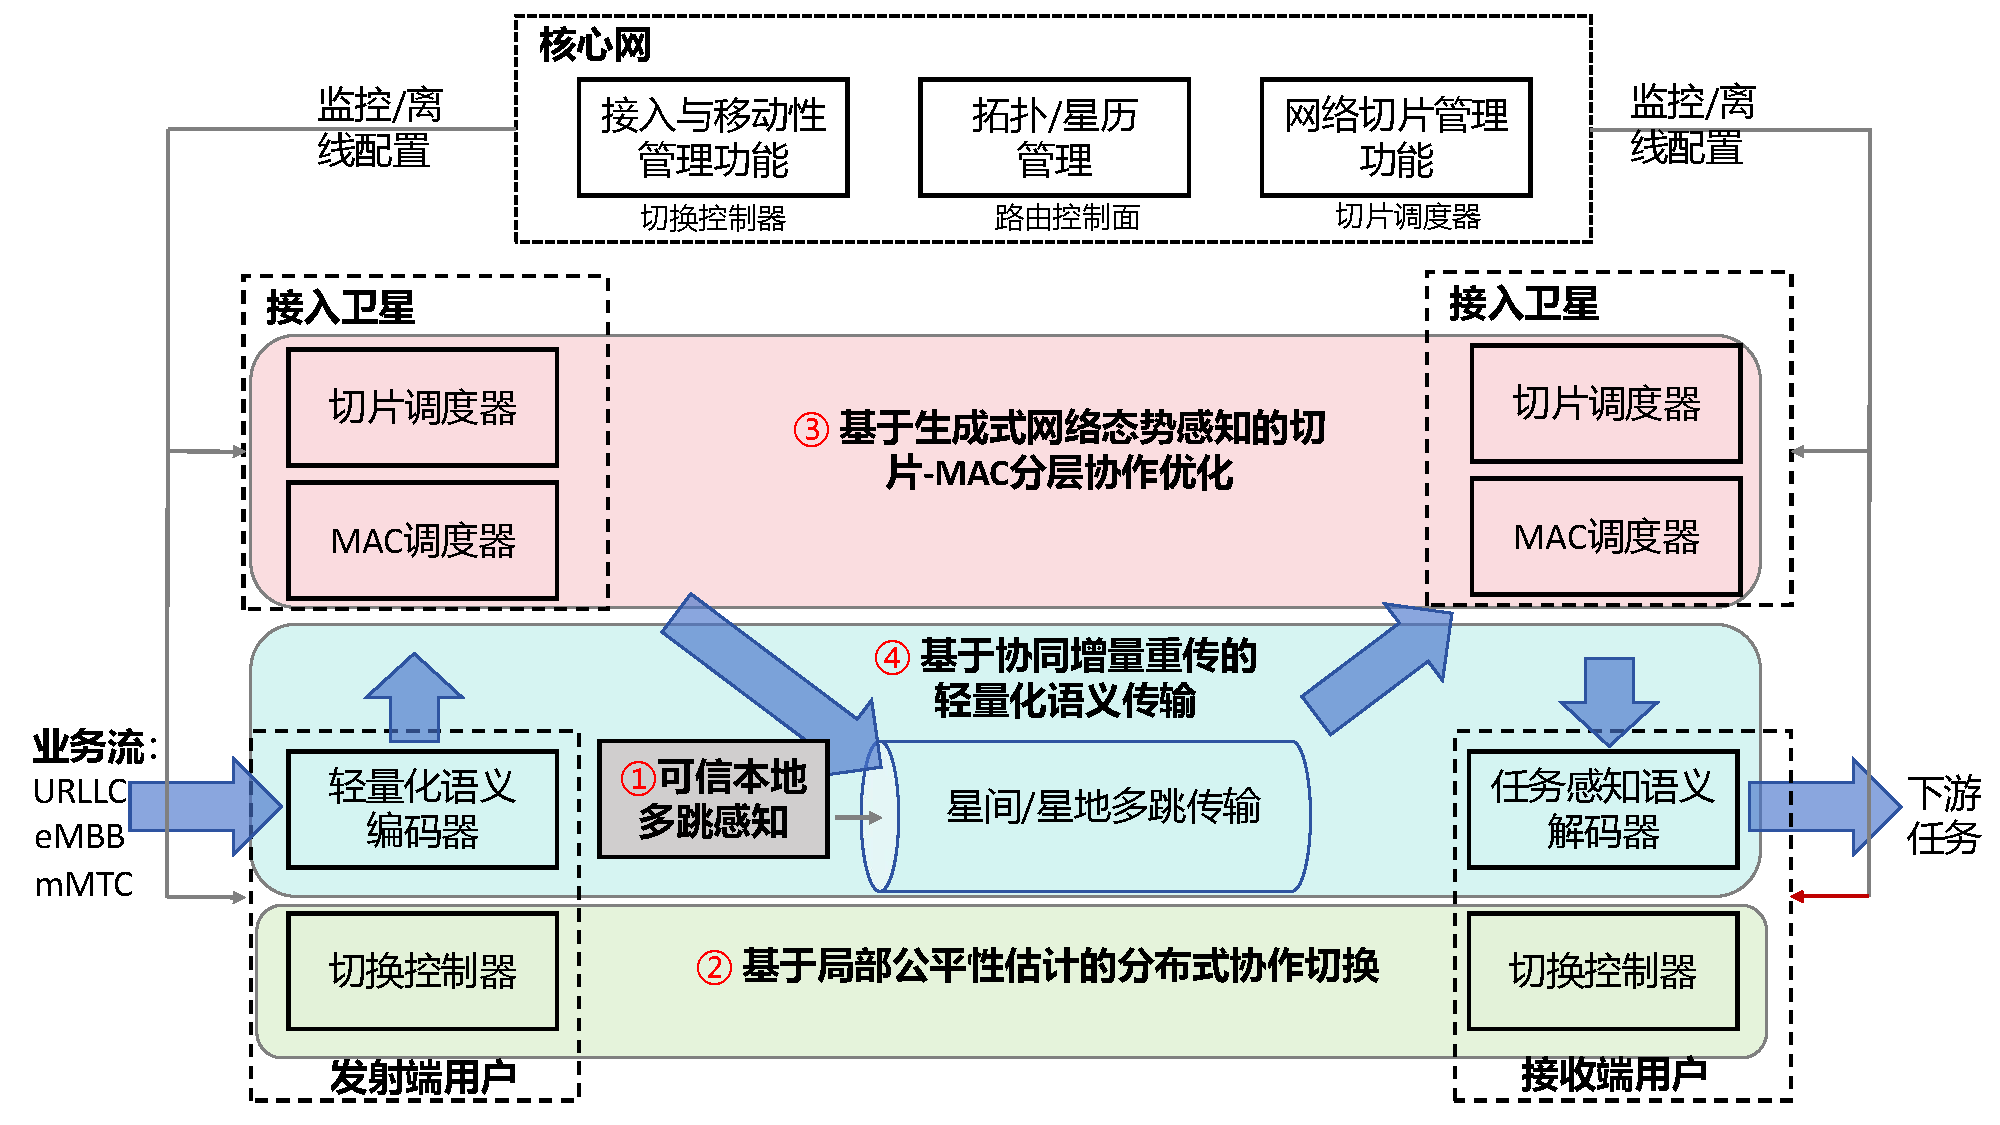
\includegraphics[width=0.9\textwidth]{figures/技术耦合.pdf}
\bicaption{四项研究内容在 LEO 卫星端到端传输系统中的部署与功能关联}
{Deployment and Functional Interrelation of the Four Research Components in the End-to-End LEO Satellite Transmission System}
\label{fig:intelligent-management-components}
\end{figure}

\textbf{（1）分布式网络状态感知}

网络状态感知位于端到端传输的决策支撑层，为星上路由、拥塞规避与资源调度提供状态输入。在纯分布式管控范式下，星上节点不依赖全网状态同步，而是在以自身为中心的有限跳邻域内获取链路负载、队列积压、信道质量与拓扑连接等网络状态信息。这些状态构成本地网络视图，是星上节点执行下一跳转发、路径选择和拥塞规避决策的直接依据。

网络状态感知的重要性在于，分布式管控决策的有效性直接取决于星上节点能否在本地获得及时、完整且可信的网络状态。在大规模 LEO 星座中，业务流经多跳星间链路转发，单颗卫星的直接观测通常仅覆盖一跳邻域，而负载均衡与拥塞规避决策需要感知下游多跳链路的剩余容量与拥塞状态。若每颗卫星都维护全网链路状态数据库，状态同步开销会随星座规模快速增长；若只使用未经校准的局部遥测，下游拥塞又可能被本地节点忽略。更为关键的是，星间链路上的状态更新与业务数据共享有限传输资源，拥塞会延迟状态更新，链路误码会造成遥测分组译码失败，使节点在决策时刻只能获得陈旧或不完整的本地视图。若这些退化状态未经校准即参与多跳特征聚合，其残余误差将作为等价路由证据向邻域传播，进而误导路径选择、模糊拥塞边界并降低多跳转发效率。

因此，网络状态感知的核心功能是在退化遥测条件下构建可信的本地多跳网络视图。具体而言，该功能需要完成三方面任务：其一，对陈旧、缺失或含噪的遥测状态进行校准，使星上节点能够基于当前物理网络状态做出决策；其二，评估校准后状态的可信度，区分由可靠观测支撑的状态与由不确定性较高的推断得到的状态；其三，以校准后置信度约束状态在多跳邻域中的传播强度，避免低可信状态作为可靠路由证据污染邻居节点的本地视图。通过上述处理，网络状态感知为后续接入切换、资源调度与可靠传输提供可靠的状态基础，是端到端管控功能链的起点。

\textbf{（2）用户接入与切换}

用户接入与切换位于端到端传输的入口环节，决定业务流能否进入空间网络并维持接入服务持续可用性。在大规模 LEO 星座中，卫星高速运动导致用户对单颗卫星的可见时间窗口通常仅为数十秒至数分钟，终端需要频繁切换接入卫星以维持与网络的连接关系。接入与切换的目标并非要求终端持续占用业务信道或连续发送数据，而是在业务服务窗口内维持有效网络附着、控制面可达性和可调度接入关联，使终端在业务数据到达时能够在可容忍时延内获得无线资源并按需恢复数据传输。

接入与切换的重要性体现在三个方面。首先，用户切换是空间控制平面中频繁发生的事件之一，高频且无效的切换会导致服务中断、端到端时延抖动以及卫星节点局部过载。其次，用户切换会直接触发回程链路调整与网络资源重新分配，进而影响端到端传输时延与网络流量分布。最后，在高动态多波束覆盖下，海量终端并发接入使相邻终端在目标卫星、随机接入资源与子信道上形成强耦合竞争。若终端仅依据瞬时信道质量独立选择接入卫星，切换请求容易向少数高增益卫星集中，引发接入负载失衡、随机接入碰撞和用户间服务质量分化，导致长期弱服务用户的卫星连接难以持续维持。

因此，用户接入与切换的核心功能是在兼顾接入服务持续可用性的同时保障系统长期用户公平性。对单个终端而言，该功能需要根据候选卫星的链路质量、剩余可见时间、接入负载以及自身业务需求，选择合适的目标卫星与子信道，并在切换过程中维持会话保持和上下文迁移；对系统而言，该功能需要通过有限邻域协作信令使相邻终端感知彼此的切换意图与长期服务状态，避免切换请求过度集中和长期欠服务用户吞吐劣化。通过上述处理，接入与切换为后续无线资源调度提供相对稳定的用户--卫星关联关系，是端到端业务承载的入口保障。

\textbf{（3）接入网无线资源调度}

接入网无线资源调度位于端到端传输的资源配置层，负责将星地频谱、发射功率与时频资源映射到已接入用户的异构业务流上。在终端与卫星建立接入关联后，业务流能否满足速率--时延门限取决于接入网能否为其分配足够的无线资源。与地面蜂窝网络类似，LEO 卫星接入网也面临频谱资源有限、发射功率受限以及多用户竞争等约束；但其资源调度问题更为复杂，原因在于星地信道高度动态、用户--卫星连接关系快速变化、业务到达随机突发以及星上计算能力受限。

无线资源调度的重要性在于，它直接决定异构业务的用户级 QoS 能否得到满足。在大规模 LEO 星座中，增强移动宽带、超可靠低时延通信和海量机器类通信等异构业务对速率、时延和可靠性提出差异化需求。传统尽力而为式调度虽可提升系统聚合吞吐量或维持队列稳定，但难以直接保障单个用户的 QoS 满足条件。网络切片可以为不同业务类别配置资源预算，但预算本身并不等价于用户级 QoS 满足：某一时刻配置的带宽和功率需要经过后续多个 MAC 时隙内的业务到达、队列竞争、信道起伏和用户连接变化后，才会体现为速率--时延门限是否被满足。若切片层资源预算决策与 MAC 层流级调度相互脱节，容易导致反应式资源配置滞后：切片层若在业务突发到来前低估资源需求，会导致后续多时隙连续违约；MAC 层若只依据瞬时信道和队列长度调度，也可能把有限资源分配给当前预算与信道条件下仍无法满足 QoS 的业务流。

因此，无线资源调度的核心功能是在资源受限和网络不确定性条件下建立资源-QoS 映射能力，使有限带宽、功率与时频资源优先服务于具备 QoS 满足条件的业务流。具体而言，该功能需要完成两方面任务：在切片层，通过前瞻性评估判断候选带宽--功率预算对未来多时隙用户级 QoS 的支撑能力，在业务突发和信道波动到来前完成资源预留；在 MAC 层，根据业务流的速率--时延需求、当前预算与信道条件判断其是否具备 QoS 可行性，并优先调度可行业务流以降低无效资源占用。通过上述处理，无线资源调度将已建立的接入连接转化为用户级资源保障能力，是端到端 QoS 保障的关键环节。

\textbf{（4）可靠传输}

可靠传输位于端到端传输的业务承载层，负责在星间/星地受限链路条件下将业务数据从源节点可靠送达目的节点。在用户获得接入连接和无线资源配置后，业务流仍需经由多跳星间承载与核心网/互联网回传链路传输至业务端。LEO 卫星网络的端到端传输面临长距离空间传播、多跳星间转发、链路高误码率以及信道状态快速变化等制约。传统比特级混合自动重传请求依赖冗余比特重传恢复错误分组，在高误码和多跳路径下容易触发多轮重传，使重传时延沿星间路径累积，并可能挤占有限星间链路资源。

可靠传输的重要性体现在两个方面。首先，端到端传输质量是用户可感知的最终服务指标，前序环节提供的接入连接与资源配置最终需要体现为业务数据的成功传输与任务相关信息的有效恢复。其次，在星上算力、星间带宽与回传容量均受限的条件下，传输机制需要在传输开销、端到端时延与任务恢复质量之间进行权衡。语义通信通过任务相关特征提取与联合信源信道编码，可在维持下游任务性能的同时降低传输资源消耗，为受限链路下的可靠传输提供跨层设计思路。然而，高性能语义模型往往需要大规模编码器与生成式解码器，难以适配受限星上载荷；轻量化模型虽可降低星上计算开销，却在低带宽、高误码条件下难以通过单次传输充分恢复任务相关语义信息。

因此，可靠传输的核心功能是在星上算力与链路带宽双重受限条件下提升任务相关信息的恢复可靠性。具体而言，该功能需要平衡三方面需求：在发送端，采用轻量化语义编码器控制星上模型复杂度与推理时延；在传输过程中，通过任务反馈引导的选择性增量重传替代完整表征重复传输，在控制附加传输开销的同时逐步提升语义恢复质量；在接收端，基于任务相关性评估语义缺口并生成紧凑反馈，引导发送端精准补充关键语义分量。通过上述处理，可靠传输在控制端到端传输时延与星上模型复杂度的同时提升受限链路下的语义传输可靠性，构成端到端业务承载的最终保障。

综上所述，网络状态感知、用户接入与切换、无线资源调度以及可靠传输四项关键技术分别作用于端到端传输的决策支撑层、入口环节、资源配置层和业务承载层，依次为星上分布式管控提供可信状态输入、接入服务持续可用性、用户级资源保障和可靠业务传输能力，共同支撑大规模 LEO 星座中的端到端 QoS 保障。


\section{基于AI的分布式管控关键技术}

\subsection{基于时空图学习的节点信息感知方法}

在基于 AI 的纯分布式网络管控架构下，星上节点不再依赖中心控制器汇聚全网状态，也不维护全网一致的链路状态数据库，而是依据本地观测与有限跳邻域状态独立完成路由转发、拥塞规避和资源调度等控制决策。由于单个节点的直接观测范围有限，仅依据本地队列、相邻链路质量和一跳邻居负载进行决策，容易忽略下游多跳链路的拥塞演化与相邻节点间的资源竞争关系，从而导致局部最优、路径震荡或链路争用冲突。因此，分布式管控中的节点信息感知不应仅停留在本地状态测量层面，而需要通过轻量级邻域协作，在控制信令开销可控的条件下构建能够近似反映全局网络状态的本地多跳视图，并为后续分布式决策提供冲突规避与协同优化依据。

考虑到 LEO 卫星网络中的邻域状态天然具有图结构特征，时空图学习为上述节点信息感知提供了一种有效实现途径\cite{zhou2021graphneuralnetworksreview}。具体而言，卫星、波束、用户或业务流可被抽象为图中的节点，星间链路、星地可见关系、候选接入关系、干扰关系或资源竞争关系可被抽象为边。节点特征可包含队列积压、业务负载、缓存状态、接入用户数、可用计算能力和历史服务水平等状态，边特征可包含链路容量、传播时延、信道质量、链路利用率、剩余可见时间和分组误码状态等属性。随着卫星轨道运动和业务流量变化，节点邻接关系、链路状态和负载分布均呈现显著的时变性，因此节点信息感知需要同时刻画空间邻接依赖与时间状态演化。

为形式化描述上述过程，记时隙 $k$ 下以管控节点 $i$ 为中心的 $h$ 跳局部邻域图为
\begin{equation}
    \mathcal G_i^h(k)=
    \big(\mathcal V_i^h(k),\mathcal E_i^h(k),
    \mathbf X_i^h(k),\mathbf E_i^h(k)\big),
\end{equation}
其中 $\mathcal V_i^h(k)$ 和 $\mathcal E_i^h(k)$ 分别表示局部邻域内的节点集合和边集合，$\mathbf X_i^h(k)=\{\mathbf x_v(k)\}_{v\in\mathcal V_i^h(k)}$ 表示节点状态特征，$\mathbf E_i^h(k)=\{\mathbf e_{uv}(k)\}_{(u,v)\in\mathcal E_i^h(k)}$ 表示边状态特征。节点信息感知的目标是在不汇聚全网状态的条件下，将局部邻域图中的节点状态、边状态和拓扑关系映射为紧凑的时空节点表征，为后续分布式资源管控提供状态输入。

从数学形式上看，图神经网络可被理解为定义在图结构上的参数共享信息聚合算子\cite{Gilmer-MessagePassingNN-ICML17,battaglia2018relationalinductivebiasesdeep}。令 $\mathbf h_v^{(0)}(k)=\rho_x(\mathbf x_v(k))$ 表示节点 $v$ 的初始状态表征，$\mathbf g_{uv}(k)=\rho_e(\mathbf e_{uv}(k))$ 表示边 $(u,v)$ 的状态表征，其中 $\rho_x(\cdot)$ 和 $\rho_e(\cdot)$ 分别为节点特征和边特征映射。第 $\ell$ 层图信息传播可写为
\begin{equation}
    \mathbf m_{u\rightarrow v}^{(\ell)}(k)
    =
    \psi_\ell
    \left(
    \mathbf h_u^{(\ell)}(k),
    \mathbf h_v^{(\ell)}(k),
    \mathbf g_{uv}(k)
    \right),
    \quad u\in\mathcal N_v(k),
\end{equation}
\begin{equation}
    \mathbf h_v^{(\ell+1)}(k)
    =
    \phi_\ell
    \left(
    \mathbf h_v^{(\ell)}(k),
    \mathrm{AGG}_\ell
    \left(
    \left\{
    \mathbf m_{u\rightarrow v}^{(\ell)}(k)
    \mid u\in\mathcal N_v(k)
    \right\}
    \right)
    \right),
\end{equation}
其中 $\mathcal N_v(k)$ 为节点 $v$ 的一跳邻居集合，$\psi_\ell(\cdot)$ 为消息生成函数，$\mathrm{AGG}_\ell(\cdot)$ 为邻居消息聚合函数，$\phi_\ell(\cdot)$ 为节点状态更新函数。该定义表明，GNN 的基本作用并非简单拼接邻居状态，而是在邻接关系约束下联合利用邻居节点状态、本节点状态和边状态。对于分布式网络管控而言，这使节点能够在有限邻域内区分不同链路质量、不同拥塞程度和不同服务可靠性的邻居状态，从而形成面向决策的局部网络态势。

若暂不显式区分边特征，上述空间聚合可写为归一化图卷积形式\cite{kipf2017semisupervisedclassificationgraphconvolutional}。记 $\mathbf A(k)$ 为时隙 $k$ 的邻接矩阵，$\widetilde{\mathbf A}(k)=\mathbf A(k)+\mathbf I$ 为加入自环后的邻接矩阵，$\widetilde{\mathbf D}(k)$ 为对应度矩阵，则一层图卷积可表示为
\begin{equation}
    \mathbf H^{(\ell+1)}(k)
    =
    \sigma
    \left(
    \widehat{\mathbf A}(k)
    \mathbf H^{(\ell)}(k)
    \mathbf W^{(\ell)}
    \right),
    \quad
    \widehat{\mathbf A}(k)
    =
    \widetilde{\mathbf D}^{-\frac{1}{2}}(k)
    \widetilde{\mathbf A}(k)
    \widetilde{\mathbf D}^{-\frac{1}{2}}(k).
\end{equation}
其中 $\mathbf H^{(\ell)}(k)$ 为第 $\ell$ 层节点表征矩阵，$\mathbf W^{(\ell)}$ 为共享参数矩阵，$\sigma(\cdot)$ 为非线性变换。该表达式说明，图卷积本质上是在既有邻接链路或资源竞争关系上进行局部状态交换与加权聚合。堆叠 $L$ 层图聚合后，节点表征最多依赖 $L$ 跳邻域内的节点和边状态。若忽略非线性变换，可近似写为
\begin{equation}
    \mathbf H^{(L)}(k)
    =
    \widehat{\mathbf A}^{L}(k)
    \mathbf X(k)
    \mathbf W .
\end{equation}
由于 $\widehat{\mathbf A}^{L}(k)$ 的第 $(v,u)$ 个元素非零仅当节点 $u$ 位于节点 $v$ 的 $L$ 跳可达邻域内，因此空间图聚合具有有限邻域感知特性\cite{Hamilton-GraphSAGE-NIPS17}。该性质与大规模 LEO 星座的分布式管控需求相匹配，即节点可以通过有限邻域协作获得多跳负载、链路余量和拥塞风险信息，同时将控制信令限制在可控范围内。

空间聚合还具有状态压缩作用。若节点 $v$ 直接收集 $L$ 跳邻域内的全部原始遥测信息，则输入维度随邻域节点数和边数增长，可近似表示为
\begin{equation}
    D_v^{\mathrm{raw}}(k)
    =
    |\mathcal B_L(v,k)|F_x
    +
    |\mathcal E_L(v,k)|F_e,
\end{equation}
其中 $\mathcal B_L(v,k)$ 为 $L$ 跳邻域节点集合，$\mathcal E_L(v,k)$ 为邻域内边集合，$F_x$ 和 $F_e$ 分别为节点特征和边特征维度。经图聚合后，节点仅需维护固定维度的空间表征
\begin{equation}
    \bar{\mathbf h}_v(k)
    =
    \mathbf h_v^{(L)}(k)
    \in\mathbb R^{F_z},
    \quad
    F_z\ll D_v^{\mathrm{raw}}(k).
\end{equation}
因此，GNN 可将多跳邻域内的队列、业务、链路、信道和可见时间等状态压缩为紧凑表征，降低分布式节点之间的状态转发开销和星上处理开销。

除空间邻域依赖外，LEO 卫星网络状态还具有显著的时间演化特征。卫星轨道运动导致星间链路和星地可见关系周期性变化，业务到达和队列积压具有时间相关性，信道质量和链路余量也会随覆盖几何关系和业务负载持续变化。因此，节点信息感知不仅需要刻画当前时隙的邻域图状态，还需要融合历史观测以判断负载增长趋势、链路退化趋势和服务质量变化趋势。

设节点 $v$ 在时隙 $k$ 由空间图聚合得到的邻域状态表征为
\begin{equation}
    \bar{\mathbf h}_v(k)
    =
    \mathrm{GNN}_{\theta}
    \left(
    \mathcal G_i^h(k),
    \mathbf X_i^h(k),
    \mathbf E_i^h(k)
    \right)_v .
\end{equation}
基于历史观测窗口 $[k-T_o,k]$，时间信息聚合可抽象表示为
\begin{equation}
    \mathbf z_v(k)
    =
    \Gamma_{\theta}
    \left(
    \bar{\mathbf h}_v(k-T_o),
    \bar{\mathbf h}_v(k-T_o+1),
    \ldots,
    \bar{\mathbf h}_v(k)
    \right),
\end{equation}
或以递推形式写为
\begin{equation}
    \mathbf z_v(k)
    =
    \Gamma_{\theta}
    \left(
    \mathbf z_v(k-1),
    \bar{\mathbf h}_v(k)
    \right),
\end{equation}
其中 $\Gamma_{\theta}(\cdot)$ 表示时间状态聚合算子，$\mathbf z_v(k)$ 表示融合空间邻域状态和历史演化状态后的时空节点表征。该表达式不限定具体实现形式，可对应循环更新或时间卷积等序列建模方式\cite{li2018diffusionconvolutionalrecurrentneural}。其共同作用是将当前邻域状态与历史状态演化相结合，使节点能够在遥测滞后、链路间歇可见和业务突发的条件下形成更稳定的网络状态感知。从时空联合建模角度看，空间聚合刻画“当前邻域内哪些节点和链路影响本节点状态”，时间聚合刻画“这些邻域状态如何随时间变化”。二者结合后，节点表征 $\mathbf z_v(k)$ 可作为路由、切换、负载均衡、资源调度和 QoS 保障等任务的统一状态输入。

基于 GNN 的表征学习还可以与图学习中的节点级、边级和图级任务形成对应关系。在节点级任务中，模型以单个节点的时空表征 $\mathbf z_v(k)$ 为输入，输出该节点相关的状态类别或连续状态量，即
\begin{equation}
    \widehat{\mathbf y}_v(k)
    =
    f_{\mathrm N}
    \left(
    \mathbf z_v(k)
    \right).
\end{equation}
当 $\widehat{\mathbf y}_v(k)$ 表示拥塞等级、接入风险等级、服务状态类别或切换风险类别时，对应节点级分类任务；当其表示未来队列长度、业务到达率、节点负载、可服务速率或 QoS 违背概率时，对应节点级回归任务。因此，节点级分类和回归可分别映射到拥塞状态识别、负载感知、流量预测和服务连续性风险感知等分布式管控功能。

在边级任务中，模型根据相邻节点表征及边状态判断链路或竞争关系的状态，即
\begin{equation}
    \widehat{\mathbf y}_{uv}(k)
    =
    f_{\mathrm E}
    \left(
    \mathbf z_u(k),
    \mathbf z_v(k),
    \mathbf e_{uv}(k)
    \right),
    \quad (u,v)\in\mathcal E(k).
\end{equation}
当输出为链路是否可用、候选下一跳是否可选、是否存在强资源竞争或是否触发链路规避时，对应边级分类任务；当输出为链路剩余容量、端到端时延贡献、丢包风险、链路利用率或剩余可见时间时，对应边级回归任务。由此，边级任务可支撑分布式路由中的候选下一跳判别、星间链路质量感知、拥塞链路规避和资源竞争关系识别。

在图级或子图级任务中，模型对一个局部区域、波束集合、覆盖区域或多跳邻域内的节点表征进行汇聚，形成区域级状态表征
\begin{equation}
    \mathbf z_{\mathcal S}(k)
    =
    \mathrm{READOUT}
    \left(
    \left\{
    \mathbf z_v(k)
    \mid v\in\mathcal V_{\mathcal S}(k)
    \right\}
    \right),
    \quad
    \widehat{\mathbf y}_{\mathcal S}(k)
    =
    f_{\mathrm G}
    \left(
    \mathbf z_{\mathcal S}(k)
    \right).
\end{equation}
其中 $\mathcal S$ 可表示一个波束覆盖区、局部星间子网、候选接入区域或资源调度区域。当输出为区域是否过载、是否存在服务失衡或是否需要触发资源重配置时，对应图级或子图级分类任务；当输出为区域总业务需求、平均服务速率、资源缺口、负载不均衡程度或长期公平性指标时，对应图级或子图级回归任务。因此，图级任务可用于支撑区域负载感知、覆盖区公平性感知、资源池容量评估和跨节点协同调度。

综上，基于时空图学习的节点信息感知可从三个层面理解。首先，在空间维度上，GNN 利用星间链路、星地可见关系、候选接入关系或资源竞争关系聚合多跳邻域状态，使分布式节点能够在有限信令开销下获得局部多跳网络视图。其次，在时间维度上，时间聚合算子利用历史观测刻画业务负载、链路质量、队列积压和服务状态的演化趋势，缓解瞬时观测不完整和遥测更新滞后带来的状态不确定性。最后，在任务维度上，节点级、边级和图级分类与回归任务分别对应拥塞识别、链路判别、路由选择、流量预测、负载感知、区域公平性感知和资源调度状态评估等网络管控功能\cite{rusek2019unveilinggnn}。由此，GNN 在分布式 LEO 卫星网络中的作用并非单纯的图结构特征提取，而是面向邻域协作、状态压缩和下游资源管控任务的通用时空状态表征基础。

\subsection{基于智能体协作的分布式资源调度方法}

大规模 LEO 卫星网络通常由成千上万颗高速运动的低轨卫星组成，星间链路、星地可见关系、业务负载和信道状态均随时间动态变化。受限于星间链路时延、星上处理能力、控制信令开销以及覆盖区域的快速切换，网络难以依赖可靠且高速的全局控制平面实时汇聚全网状态并统一下发资源调度决策。因此，面向大规模 LEO 卫星网络的在线资源管控需要从传统集中式优化转向分布式协作模式，即由邻近卫星、波束或接入节点形成局部自治域，在有限信息交互条件下自主完成业务感知、资源协调、干扰规避和负载均衡等调度功能。多智能体强化学习为上述分布式资源调度提供了一种有效的理论基础，使多个智能体能够在共享网络环境中依据局部观测、邻域交互和资源调度反馈形成协作决策能力\cite{huh2024multiagentreinforcementlearningcomprehensive}。在 LEO 卫星网络中，可将卫星节点、波束控制器、接入节点或局部调度单元抽象为智能体，将链路带宽、发射功率、时频资源、缓存空间和星上计算能力等抽象为可调度资源，从而通过多智能体协作实现分布式在线资源管控。

从数学形式上看，分布式资源调度过程可被描述为部分可观测的多智能体马尔可夫决策过程，其基本形式可写为
\begin{equation}
    \mathcal M=
    \left(
    \mathcal I,\mathcal S,
    \{\mathcal O_i\}_{i\in\mathcal I},
    \{\mathcal A_i\}_{i\in\mathcal I},
    P,\{r_i\}_{i\in\mathcal I},\gamma
    \right),
\end{equation}
其中 $\mathcal I=\{1,\ldots,N\}$ 表示智能体集合，$\mathcal S$ 表示全局网络状态空间，$\mathcal O_i$ 和 $\mathcal A_i$ 分别表示智能体 $i$ 的局部观测空间和动作空间，$P$ 表示网络状态转移关系，$r_i$ 表示智能体 $i$ 获得的调度反馈，$\gamma\in[0,1)$ 为折扣因子。该形式可视为随机博弈模型在分布式网络管控中的表达，其中多个智能体在同一网络环境中同时执行动作，并共同影响后续链路状态、队列状态和资源占用状态\cite{sutton1998reinforcementlearning}。

在时隙 $k$，智能体 $i$ 根据局部观测 $\mathbf o_i(k)$ 选择资源调度动作
\begin{equation}
    a_i(k)\sim \pi_i\left(\cdot\mid \mathbf o_i(k)\right),
\end{equation}
所有智能体的动作组成联合动作
\begin{equation}
    \mathbf a(k)=\left(a_1(k),a_2(k),\ldots,a_N(k)\right).
\end{equation}
随后，网络状态按照
\begin{equation}
    s(k+1)\sim P\left(\cdot\mid s(k),\mathbf a(k)\right)
\end{equation}
进行演化，并向各智能体返回相应调度反馈 $r_i(k)$。智能体的目标是在长期交互过程中形成策略 $\pi_i$，使其在局部观测受限的条件下提升长期资源利用效率、业务服务质量和邻域协作性能。由于 LEO 卫星网络难以实时获取完整全局状态，智能体策略在执行阶段通常只能依赖本地状态、邻域状态和有限交互信息，而不能依赖全网集中式控制信息。

在分布式资源调度中，局部观测 $\mathbf o_i(k)$ 的设计应体现“本地可测、邻域可交互、任务相关、开销可控”的原则。一般可将智能体 $i$ 的观测表示为
\begin{equation}
    \mathbf o_i(k)=
    \left[
    \mathbf o_i^{\mathrm{loc}}(k),
    \mathbf o_i^{\mathrm{nei}}(k),
    \mathbf o_i^{\mathrm{qos}}(k),
    \mathbf o_i^{\mathrm{msg}}(k)
    \right],
\end{equation}
其中 $\mathbf o_i^{\mathrm{loc}}(k)$ 表示本地资源与业务状态，例如本地队列长度、缓存占用、可用带宽、剩余功率、可用计算能力和当前接入用户数；$\mathbf o_i^{\mathrm{nei}}(k)$ 表示有限跳邻域状态，例如相邻链路质量、邻居负载、候选下一跳状态、干扰关系和邻域资源占用情况；$\mathbf o_i^{\mathrm{qos}}(k)$ 表示业务服务状态，例如时延约束、丢包风险、服务连续性风险和用户公平性状态；$\mathbf o_i^{\mathrm{msg}}(k)$ 表示来自邻居智能体的压缩协作信息。上一小节中的时空图节点表征 $\mathbf z_i(k)$ 也可作为 $\mathbf o_i^{\mathrm{nei}}(k)$ 或 $\mathbf o_i^{\mathrm{msg}}(k)$ 的一种紧凑表示，从而避免在强化学习决策阶段重复传输高维原始遥测信息。

动作空间应根据具体资源调度对象区分离散动作、连续动作以及混合动作。对于路由下一跳选择、候选接入卫星选择、波束选择、信道块选择、用户调度顺序和切换触发判决等问题，动作通常表现为离散动作，可表示为
\begin{equation}
    a_i^{\mathrm d}(k)\in\mathcal A_i^{\mathrm d}(k).
\end{equation}
对于功率控制、带宽比例分配、时频资源占比、计算资源分配、缓存空间分配和语义压缩率控制等问题，动作通常表现为连续动作，可表示为
\begin{equation}
    \mathbf a_i^{\mathrm c}(k)\in\mathcal A_i^{\mathrm c}(k).
\end{equation}
在实际网络资源管控中，离散动作和连续动作往往同时存在，因此可将智能体动作统一表示为
\begin{equation}
    a_i(k)=
    \left(
    a_i^{\mathrm d}(k),
    \mathbf a_i^{\mathrm c}(k)
    \right),
\end{equation}
其中离散部分决定资源调度对象或调度模式，连续部分决定资源分配比例或控制参数。无论动作空间采用何种形式，动作设计均应满足物理链路约束、功率约束、带宽约束、可见性约束和星上处理能力约束；对于不可行动作，应通过动作掩码、可行域约束或动作投影等方式保证策略输出不会破坏通信资源约束。

奖励反馈用于刻画智能体动作对网络运行状态的影响，其设计应同时反映个体调度收益和邻域协作影响。一般可将智能体 $i$ 的奖励写为
\begin{equation}
    r_i(k)
    =
    u_i^{\mathrm{svc}}(k)
    -
    c_i^{\mathrm{qos}}(k)
    -
    c_i^{\mathrm{res}}(k)
    -
    c_i^{\mathrm{conf}}(k)
    +
    u_i^{\mathrm{coop}}(k),
\end{equation}
其中 $u_i^{\mathrm{svc}}(k)$ 表示业务服务收益，可对应吞吐量提升、成功传输分组数或有效服务用户数；$c_i^{\mathrm{qos}}(k)$ 表示 QoS 代价，可对应时延违约、丢包、链路中断或切换失败；$c_i^{\mathrm{res}}(k)$ 表示资源消耗代价，可对应功率消耗、带宽占用、缓存占用或计算开销；$c_i^{\mathrm{conf}}(k)$ 表示决策冲突代价，可对应干扰增强、链路争用、重复调度或邻居拥塞外溢；$u_i^{\mathrm{coop}}(k)$ 表示协作收益，可对应负载均衡、区域公平性提升或邻域拥塞缓解。奖励设计不应只鼓励单个节点的瞬时吞吐最大化，还应抑制自私抢占资源、局部链路过载和跨节点决策冲突，使局部学习目标与网络整体服务目标保持一致。

在训练范式方面，集中训练分布执行是一类适合大规模网络离线训练和在线部署相结合的通用方法\cite{kraemer2016multiagentreinforcementlearning}。其核心思想是在训练阶段允许利用更完整的网络状态、联合动作、邻域反馈或仿真轨迹，以缓解多智能体同时学习带来的环境非平稳性和协作信用分配困难；但在执行阶段，每个智能体仍只依据本地观测和邻域交互信息独立输出动作，即
\begin{equation}
    a_i(k)\sim\pi_i\left(\cdot\mid \mathbf o_i(k)\right).
\end{equation}
因此，CTDE 并不要求在实际运行时部署中心控制器，也不要求在线收集全局状态，而是将集中信息主要用于训练阶段的策略评估、经验复用或离线预训练。对于 LEO 卫星网络，该范式适合在数字孪生环境、地面训练平台或历史遥测数据集上学习协作策略，再将局部策略部署到星上节点或边缘调度单元中执行。

与 CTDE 不同，完全分布式训练与执行要求智能体在训练和执行阶段均不依赖全局状态、集中式价值评估器或中心参数更新器。每个智能体仅基于自身观测、局部奖励、邻域消息和有限历史经验更新策略，可表示为
\begin{equation}
    \pi_i:
    \left(
    \mathbf o_i(k),
    \{\mathbf m_{j\rightarrow i}(k)\}_{j\in\mathcal N_i^{\mathrm c}(k)}
    \right)
    \mapsto a_i(k),
\end{equation}
其中 $\mathcal N_i^{\mathrm c}(k)$ 表示智能体 $i$ 在通信约束下可交换信息的邻居集合，$\mathbf m_{j\rightarrow i}(k)$ 表示邻居智能体 $j$ 发送的协作消息。完全分布式训练更符合星间控制平面不稳定、跨域回传受限和在线自适应需求较强的场景，但也更容易受到部分可观测、样本效率低、非平稳学习和智能体间误协调的影响\cite{zhang2018fullydecentralizedmultiagentreinforcement}。因此，在该范式下，观测设计、奖励设计和邻域消息设计需要更加谨慎，应尽量通过有限邻域信息交换、同构节点参数共享、局部模型同步或协作约束来提升策略稳定性和可迁移性。

综上，基于智能体协作的分布式资源调度方法可从三个层面理解。首先，在决策建模层面，LEO 卫星网络中的分布式资源调度可被建模为部分可观测的多智能体马尔可夫决策过程，智能体在局部观测和邻域交互条件下共同影响网络状态演化。其次，在资源管控层面，观测、动作和奖励应分别围绕业务状态感知、资源调度行为和网络服务目标进行设计，并兼顾链路约束、QoS 保障、资源利用效率和邻域协作关系。最后，在训练部署层面，CTDE 适合利用离线全局信息提升训练稳定性并支持分布式执行，而完全分布式训练更适合在缺乏可靠控制平面的星上自治场景中进行在线自适应。由此，多智能体强化学习为大规模 LEO 卫星网络中的分布式路由、接入切换、负载均衡、功率控制和无线资源调度提供了统一的协作决策基础。

\section{本章小结}

本章面向大规模 LEO 卫星网络的分布式管控需求，系统分析了集中式、传统分布式和基于 AI 的纯分布式三类典型管控架构，并以星间路由为例说明了不同架构在控制闭环位置、状态视图范围和状态同步开销方面的差异。随后，本章从端到端传输系统出发，梳理了网络状态感知、用户接入与切换、无线资源调度和可靠传输四项关键技术在业务承载流程中的部署位置与功能关系。进一步地，本章介绍了基于时空图学习的节点信息感知方法和基于智能体协作的分布式资源调度方法，说明了图结构状态表征与多智能体协作决策在纯分布式管控中的基础作用。上述内容为后续章节围绕可信状态感知、分布式接入切换、用户级资源保障和语义可靠传输展开具体方法设计提供了统一的架构背景与技术主线。